\section{Grundlagen von Netzwerkhacks}
Um ein gewisses Grundwissen über die Vorgehensweise von Hackern zu erhalten werden in diesem Kapitel die Grundlagen von Angriffen, die über ein Netzwerk stattfinden, genauer erläutert. Mit diesem Wissen können später die vom Honeypot aufgezeichneten Log-Dateien ausgewertet werden.
Zunächst werden kurz die Grundlagen der netzbasierten Kommunikation, danach verschiedene Angriffsszenarien genauer betrachtet.  

\subsection{Netzkommunikation}
Die Kommunikation in einem Netzwerk findet über s.g. Netzprotokolle statt. So wird gewährleistet, dass der Sender und der Empfänger die selbe "Sprache" sprechen. Wird z.B. eine Web Seite in einem Browser aufgerufen, wir meist das HTTP-Protokoll verwendet. Dieses wird über weitere Protokolle in ein Paket gepackt, und an den gewünschten Web Server gesendet. Dieser entpackt das Paket in umgekehrter Reihenfolge wie der Sender, und gelangt so letztendlich zur ursprünglichen Nachricht\cite{tannensbaum.2012a}. Für die Reihenfolge der anzuwendenden Protokolle gibt es zwei Grundlegende Referenzmodelle:\\
\\
\noindent\textbf{OSI-Referenzmodell}\\
\noindent Das  OSI-Schichtenmodell beschreibt die Struktur der gesamten Kommunikation zweier Kommunikationsteilnehmer. Es besteht aus sieben Schichten, die aus jeweils mehreren Protokollen bestehen, die für unterschiedliche Aufgabenstellungen zuständig sind\cite{tannensbaum.2012a}:\\
\begin{itemize}
\item Anwendungsschicht: Diese Schicht sorgt für eine Umsetzung der Anforderungen der Anwendung
\item Darstellungsschicht: Diese Schicht sorgt dafür das die Nachricht in eine für die Anwendung verwertbare Sprache zur Verfügung gestellt wird
\item Kommunikationsschicht: Diese Schicht kümmert sich um den Aufbau und Überwachung von Verbindungen
\item Transportschicht: Diese Schicht sorgt für eine transparente Ende-zu-Ende Verbindung mit einem Kommunikationspartner
\item Vermittlungsschicht: Die Vermittlungsschicht kümmert sich um die Vermittlung der oberen Schichten. Zu ihren Aufgaben gehören unter anderem das Routing und die Adressierung.
\item Sicherungsschicht: Diese Schicht bietet Funktionen wie Fehlerkorrekturen und Flusssteuerung an
\item Bitübertragungsschicht: Die unterste Schicht behandelt die physikalische Verbindung zweier Punkte und ist für die Bitstream-Übertragung zuständig 
\end{itemize}

\noindent Die Kommunikation über diese Schichten findet über Paketen statt, die z.B. in der Anwendungsschicht erstellt, und danach in die darauf folgenden sechs Schichten gekapselt verpackt werden. Beim Empfänger werden die Schichten zur Anwenderschicht wieder entfernt bis die eigentliche Nachricht interpretierbar wird. In Abb. \ref{osi} wird ein Beispielkommunikation über das Internet dargestellt.\\
\begin{figure}[h]
    \centering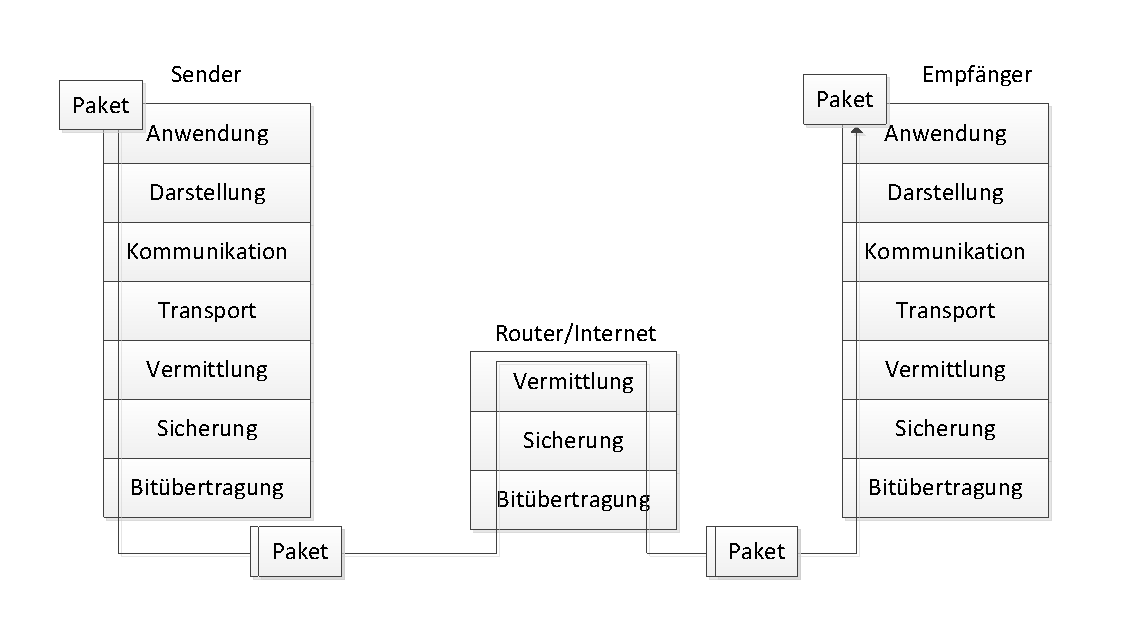
\includegraphics[scale=0.7]{Bilder/OSI.pdf}
  \caption{Kommunikation über das OSI-Schichtenmodell}
  \label{osi}
\end{figure}

\noindent Das OSI-Schichtenmodell wir häufig als Grundlage für den Entwurf neuer Netzwerkprotokolle verwendet. In der Realität finden Kommunikation meist über weniger Schichten statt, wie z.B. das TCP/IP-Referenzmodell.\\

\noindent\textbf{TCP/IP-Referenzmodell}\\
\noindent Das TCP/IP-Referenzmodell basiert auf dem OSI-Modell, fasst jedoch die Aufgaben einiger Schichten zusammen. So wird satt der Bitübertragungs- und Sicherungsschicht eine allgemeine Netzzugangsschicht, und aus Kommunikations-, Darstellungs-, und Anwendungsschicht eine allgemeine Anwendungsschicht. Die Vermittlungs-, und Transportschicht werden beibehalten. \\

\subsection{Netzwerkprotokolle}
Netzwerkprotokolle besitzen je nach Zweck und Netzwerkschicht verschieden Merkmale und Funktionen. Viele Netzwerkprotokolle hängen von der obersten Schicht bis zur Untersten einen eigenen Protokoll Header an. Dieser besitzt wichtige Merkmale zum Transport der darauf folgenden Daten. Einige der wichtigsten Protokolle und deren Header Funktionen werden in diesem Kapitel genauer betrachtet:\\
\\
\begin{itemize}
\item IP: Das Internet Protocol ist ein sehr weit verbreitetes Netzwerkprotokolle welches die Grundlagen des Internet darstellt. Es befindet sich in der Vermittlungsschicht des OSI-Schichtenmodells und ist somit für die Vermittlung über IP-Adressen zuständig.  
\item TCP: Das Transmission Control Protocol ist ein Netzwerkprotokoll der Transportschicht. Dieses garantiert eine zuverlässige, verbindungsorientierte Transport von Paketen in Computernetzwerken. Es zählt wie das IP-Protokoll zu den Grundlagen des Internets. In diesem Protokoll-Header werden der Quell und Ziel Port genannt, um dem meist zuvor erstellten IP-Paket einen bestimmten Dienst zuzuweisen. Eine TCP-Verbindung erfolgt immer über eine vorgegebene Startsequenz. Diese wird 3-Way-Handshake genannt und wir in Abb. \ref{3way} dargestellt. Dabei werden die Control-Flag-Bits im Header jeweils geändert. 

\begin{figure}[h]
    \centering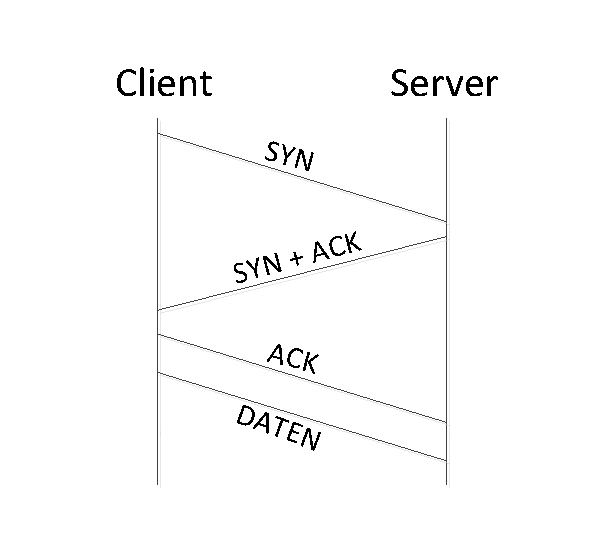
\includegraphics[scale=0.7]{Bilder/3way.pdf}
  \caption{Drei-Wege-Handshake mit TCP}
  \label{3way}
\end{figure}

Nach dem Aufbau der Verbindung können Daten gesendet werden.

\item UDP: Beim User Datagram Protocl handelt es sich um ein verbindungsloses Transportprotokoll. Wie bei TCP befindet sich in seinem Header Ziel- und Quell-Port, jedoch erfolgt kein Verbindungsaufbau. Außerdem wird nicht überprüft, ob alle Pakete tatsächlich beim Benutzer ankommen. 
\item HTTP/HTTPS:Das Hyper Text Transfer Protocol wird von Web-Servern verwendet, um deren Webseiten an den Benutzer zu senden. Diese Protokoll befindet sich bereits in der Anwenderschicht, und baut auf einer TCP/IP Verbindung auf.
\item SSH: Das Secure Shell Protokoll ist ein Netzwerkprotokoll, welches sich ebenfalls auf der Anwenderschicht befindet. Es öffnet eine verschlüsselte Verbindung auf einen entfernten Server, um die Kommandozeile dessen lokal zur Verfügung zu stellen. 
\item FTP: Das File Transfer Protocol wird zur Übertragung von Daten allgemein verwendet. Das Anwendungsprotokoll wird verwendet um vom Server Daten herunter- oder hochzuladen. 
\end{itemize}

\noindent Die Protokolle die in den jeweiligen Schichten angewendet werden, sind oft Angriffsziel vieler Hacker. Diese können über bewusste Manipulation so abgeändert werden, dass das System oft unerwartet reagiert. Einige mögliche Angriffsszenarien werden im folgenden Kapitel betrachtet. 
